\subsection{Scenario 3}

\subsubsection{Configuration}

Pour voir ce qui se passe au niveau du contrôleur, on pourra si on le souhaite lancer une session wireshark sur l'interface concernée afin d'examiner les divers paquets Openflow transitant entre ONOS et switchs (notamment les paquets encapsulés en PACKET\_IN). Le filtre "tcp.port == 6633 \&\& openflow\_v4 \&\& (openflow\_v4.type == OFPT\_PACKET\_IN or openflow\_v4.type == OFPT\_PACKET\_OUT)" peut être utilisé pour supprimer les paquets inutiles.
Exécuter les instructions suivantes dans la console Mininet après avoir lancé le fichier general\_topology.py :

\begin{minted}{bash}
$ sudo ./general_topology.py [addresse IP du contrôleur]
$> h11 python scenario3/packet_in_flooding.py 06:06:06:06:06:06 h11-eth0 &
$> iperf h1 h8
$> iperf h4 h8
$> iperf h12 h8
\end{minted}

Attendre quelques secondes entre les 2 premières commandes, le temps que les tables de flux du switch associé à h8 se chargent (sinon l'attaque fonctionne moins bien : la nouvelle règle correspondant au ping est plus utilisée que les règles aléatoires inutiles, donc va accroître sa priorité au fur et à mesure que certaines des règles aléatoires de priorité plus grande vont disparaître puisqu'inusitées).


\subsubsection{Résultat}

\begin{figure}[h]
  	\centering
  	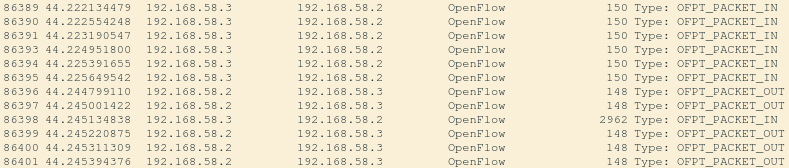
\includegraphics[width=1\textwidth]{packets_in.png}
  	\caption{Nombreux PACKET\_IN et PACKET\_OUT dans ONOS}
\end{figure}

Sous wireshark, on observe l'échange de nombreux PACKET\_IN et PACKET\_OUT avec le switch malveillant.

\begin{figure}[h]
  	\centering
  	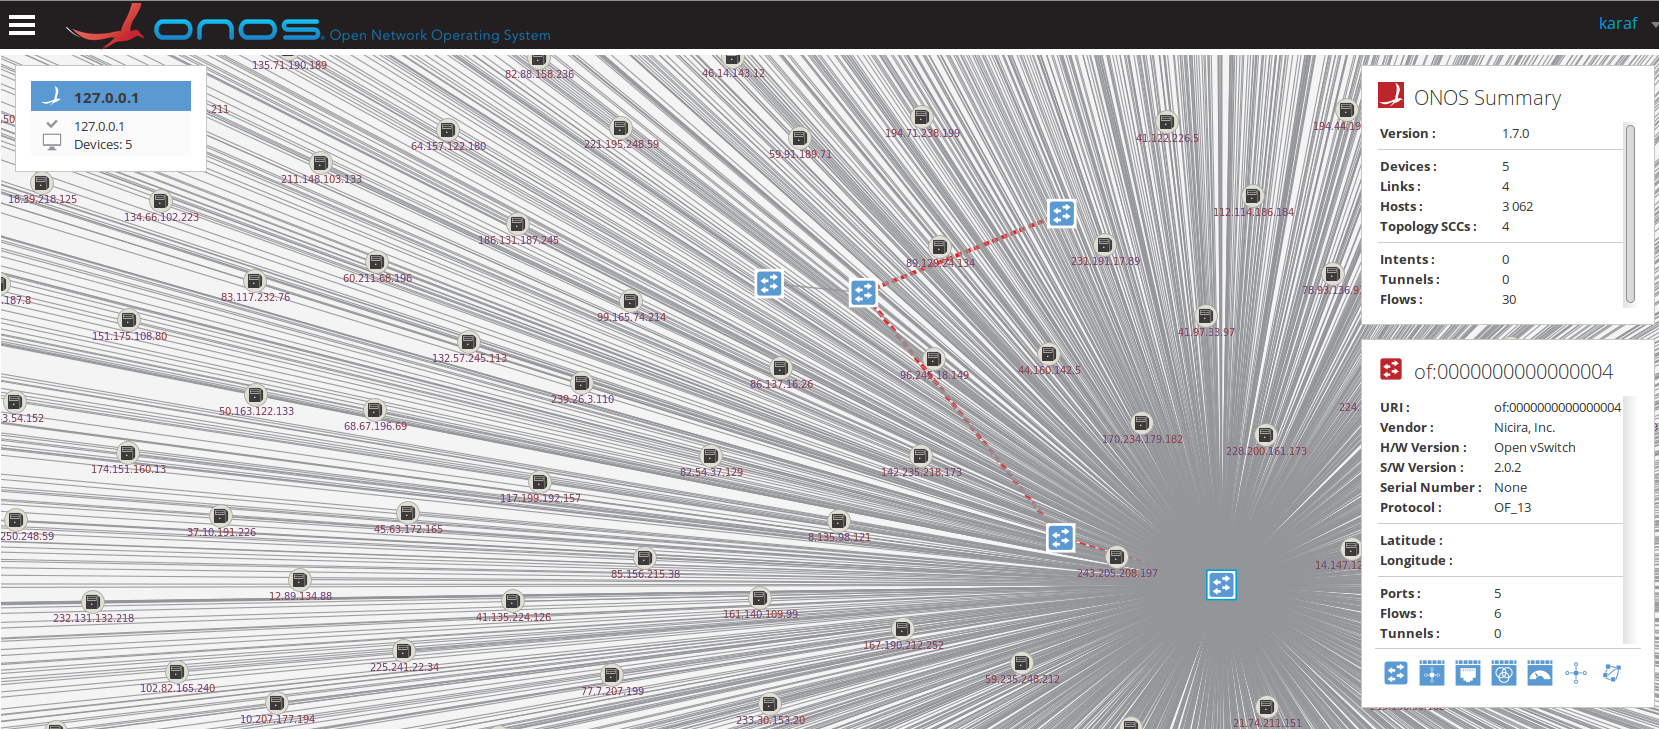
\includegraphics[width=1\textwidth]{surcharge.png}
  	\caption{Réseau attaqué : beaucoup d'hôtes sont détectés par ONOS}
\end{figure}

\begin{figure}[h]
  	\centering
  	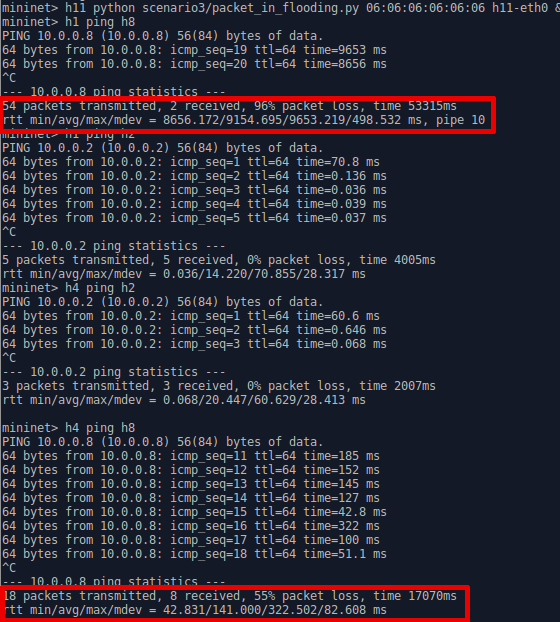
\includegraphics[width=0.8\textwidth]{DOS.png}
  	\caption{Réseau attaqué : ping beaucoup plus faible, perte de paquets}
\end{figure}

\underline{Conclusion :}\\
